\documentclass[11pt,letterpaper]{article}

\usepackage[utf8]{inputenc}
\usepackage{fullpage} % Package to use full page
\usepackage{parskip} % Package to tweak paragraph skipping
\usepackage{tikz} % Package for drawing
\usepackage{amsmath}
\usepackage{amsfonts}
\usepackage[utf8]{inputenc}
\usepackage{fullpage} % Package to use full page
\usepackage{parskip} % Package to tweak paragraph skipping
\usepackage{tikz} % Package for drawing
\usepackage{amsmath}
\usepackage{amsfonts}
\usepackage{amssymb}
\usepackage{hyperref}
\usepackage{float}
\usepackage[]{algorithm2e}
\usepackage{listings}
\usepackage{tabularx}
\usepackage{tikz}
\usepackage[spanish,es-nodecimaldot]{babel}
\newcommand{\shellcmd}[1]{\\\indent\indent\texttt{\footnotesize\# #1}\\}

\title {Facultad de Ciencias, UNAM\\
Creación e implementación de un protocolo de la capa de Aplicación\\  
Redes de Computadoras
		}
\author{Marisol Amézcua Lopez}  

\date{\today}  

\begin{document}

\maketitle

Objetivo: Implementar una aplicación que dada una base de datos con items y usuarios sea posible tener un registro de los items de cada usuario así como poder capturar nuevos items y registrarlos en el historial del usuario. 

El autómata de la aplicación es el siguiente:

\begin{center}
	\begin{tikzpicture}[scale=0.2]
	\tikzstyle{every node}+=[inner sep=0pt]
	\draw [black] (12.1,-8.1) circle (3);
	\draw (12.1,-8.1) node {$S_0$};
	\draw [black] (27,-8.1) circle (3);
	\draw (27,-8.1) node {$S_{11}$};
	\draw [black] (40.5,-8.1) circle (3);
	\draw (40.5,-8.1) node {$S_{22}$};
	\draw [black] (54.6,-8.1) circle (3);
	\draw (54.6,-8.1) node {$S_3$};
	\draw [black] (67.5,-8.1) circle (3);
	\draw (67.5,-8.1) node {$S_4$};
	\draw [black] (12.1,-18.8) circle (3);
	\draw (12.1,-18.8) node {$S_{12}$};
	\draw [black] (12.1,-29.7) circle (3);
	\draw (12.1,-29.7) node {$S_{21}$};
	\draw [black] (27,-29.7) circle (3);
	\draw (27,-29.7) node {$F$};
	\draw [black] (47.7,-23.8) circle (3);
	\draw (47.7,-23.8) node {$S_5$};
	\draw [black] (12.1,-11.1) -- (12.1,-15.8);
	\fill [black] (12.1,-15.8) -- (12.6,-15) -- (11.6,-15);
	\draw (11.6,-13.45) node [left] {$43$};
	\draw [black] (15.1,-8.1) -- (24,-8.1);
	\fill [black] (24,-8.1) -- (23.2,-7.6) -- (23.2,-8.6);
	\draw (19.55,-8.6) node [below] {$10$};
	\draw [black] (12.1,-21.8) -- (12.1,-26.7);
	\fill [black] (12.1,-26.7) -- (12.6,-25.9) -- (11.6,-25.9);
	\draw (11.6,-24.25) node [left] {$44$};
	\draw [black] (27,-11.1) -- (27,-26.7);
	\fill [black] (27,-26.7) -- (27.5,-25.9) -- (26.5,-25.9);
	\draw (26.5,-18.9) node [left] {$41/42$};
	\draw [black] (30,-8.1) -- (37.5,-8.1);
	\fill [black] (37.5,-8.1) -- (36.7,-7.6) -- (36.7,-8.6);
	\draw (33.75,-8.6) node [below] {$20$};
	\draw [black] (38.91,-10.64) -- (28.59,-27.16);
	\fill [black] (28.59,-27.16) -- (29.44,-26.74) -- (28.59,-26.21);
	\draw (33.12,-17.61) node [left] {$32$};
	\draw [black] (43.5,-8.1) -- (51.6,-8.1);
	\fill [black] (51.6,-8.1) -- (50.8,-7.6) -- (50.8,-8.6);
	\draw (47.55,-8.6) node [below] {$30$};
	\draw [black] (56.158,-5.565) arc (135.82817:44.17183:6.82);
	\fill [black] (65.94,-5.56) -- (65.74,-4.64) -- (65.03,-5.34);
	\draw (61.05,-3) node [above] {$21$};
	\draw [black] (65.848,-10.576) arc (-46.12169:-133.87831:6.922);
	\fill [black] (56.25,-10.58) -- (56.48,-11.49) -- (57.18,-10.77);
	\draw (61.05,-13.01) node [below] {$30$};
	\draw [black] (52.24,-9.95) -- (29.36,-27.85);
	\fill [black] (29.36,-27.85) -- (30.3,-27.75) -- (29.68,-26.96);
	\draw (38.02,-18.4) node [above] {$42/23$};
	\draw [black] (53.39,-10.85) -- (48.91,-21.05);
	\fill [black] (48.91,-21.05) -- (49.69,-20.52) -- (48.77,-20.12);
	\draw (50.42,-14.97) node [left] {$22$};
	\draw [black] (44.81,-24.62) -- (29.89,-28.88);
	\fill [black] (29.89,-28.88) -- (30.79,-29.14) -- (30.52,-28.18);
	\draw (36.14,-26.17) node [above] {$32$};
	\draw [black] (67.328,-11.093) arc (-6.59655:-117.25847:26.007);
	\fill [black] (29.58,-31.22) -- (30.06,-32.04) -- (30.52,-31.15);
	\draw (55.22,-31.56) node [below] {$31$};
	\draw [black] (15.1,-29.7) -- (24,-29.7);
	\fill [black] (24,-29.7) -- (23.2,-29.2) -- (23.2,-30.2);
	\draw (19.55,-30.2) node [below] {$\varepsilon$};
	\end{tikzpicture}
\end{center}

\begin{tabular}{|c|c|}
	\hline 
	Codigo  & Descripción \\ 
	\hline 
	10 & Se solicita al servidor capturar un pokemon \\ 
	\hline 
	20 & Desea capturar al pokemon x? \\ 
	\hline 
	21 & Desea volver a capturar al pokemon x? Le quedan k intentos \\ 
	\hline 
	22 & Felicidades, capturaste al pokemon x. Despliega imagen de pokemon x. \\ 
	\hline 
	23 & Número de intentos agotados. \\ 
	\hline 
	30 & Sí \\ 
	\hline 
	32 & Terminando sesión/No \\ 
	\hline 
	41 & Error con el id que ingreso el usuario. \\ 
	\hline 
	42 & Codigo de error interno en algun punto \\ 
	\hline 
	43 & Se solicita al servidor desplegar la pokedex \\ 
	\hline 
	44 & Pokedex obtenida exitosamente. Se despliegan los nombres de los pokemones capturados. \\ 
	\hline 
\end{tabular} 

{\tiny Nota: En el código 32 se englobo el 31 y 32 debido a que no aportaba ningún cambio el 31.}

La estructura de los mensajes es el siguiente:

\begin{itemize}
	\item Los mensajes de los códigos 23,30,32,41,42 y 44 constan de un solo byte.
	
	$\underset{1 byte}{\begin{tabular}{|c|}
		\hline 
		codigo \\ 
		\hline 
		\end{tabular}} $
	
	\item El mensaje para el codigo 10 y 43 consta de un byte para el numero de codigo y un byte para el id del usuario:
	
	$\underset{1 byte}{\begin{tabular}{|c|}
		\hline 
		codigo \\ 
		\hline 
		\end{tabular}}\underset{1 byte}{\begin{tabular}{|c|}
		\hline 
		id\_usuario \\ 
		\hline 
		\end{tabular}} $
	\item El mensaje para el codigo 20 consta de un byte seguido de un byte para la cantidad de bytes del nombre del pokemon y al final esta el nombre del mismo:
	
	$\underset{1 byte}{\begin{tabular}{|c|}
		\hline 
		codigo \\ 
		\hline 
		\end{tabular}}\underset{1 byte}{\begin{tabular}{|c|}
		\hline 
		k \\ 
		\hline 
		\end{tabular}}\underset{k bytes}{\begin{tabular}{|c|}
		\hline 
		nombre\_pokemon \\ 
		\hline 
		\end{tabular}} $
	\item El mensaje 21 consta de 1 byte para el codigo y otro para el numero de intentos restantes:
	
	$\underset{1 byte}{\begin{tabular}{|c|}
		\hline 
		codigo \\ 
		\hline 
		\end{tabular}}\underset{1 byte}{\begin{tabular}{|c|}
		\hline 
		intentos \\ 
		\hline 
		\end{tabular}} $
	
	\item El mensaje 22 contiene 1 byte para el codigo, 4 bytes para el tamaño de la imagen y k bytes para el tamaño de la imagen.
	
	$\underset{1 byte}{\begin{tabular}{|c|}
		\hline 
		codigo \\ 
		\hline 
		\end{tabular}}\underset{1 byte}{\begin{tabular}{|c|}
		\hline 
		k \\ 
		\hline 
		\end{tabular}}\underset{k bytes}{\begin{tabular}{|c|}
		\hline 
		tamaño\_imagen \\ 
		\hline 
		\end{tabular}} $
	
	\item El codigo 44 contiene 1 byte para el numero de código, 1 byte para el tamaño del string que representa la pokedex y k bytes que son la pokedex: 
	
	
	$\underset{1 byte}{\begin{tabular}{|c|}
		\hline 
		codigo \\ 
		\hline 
		\end{tabular}}\underset{1 byte}{\begin{tabular}{|c|}
		\hline 
		k \\ 
		\hline 
		\end{tabular}}\underset{k bytes}{\begin{tabular}{|c|}
		\hline 
		tamaño\_pokedex \\ 
		\hline 
		\end{tabular}} $
\end{itemize}


{\tiny Nota: A algunos codigos se les cambiaron el número de bytes para facilitar la implementación.}

\section{Uso de la aplicación}

En ambos casos lo primero es correr el servidor, para esto es necesario ejecutar el comando

\textsf{python3 server.py $<$IP$>$ $<$Puerto$>$}

Si todo sale bien veremos un mensaje de que el servidor se encuentra escuchando el puerto, en otro caso veremos un mensaje de error.

%Imagen de run server
\begin{figure}[h!]
	\centering
	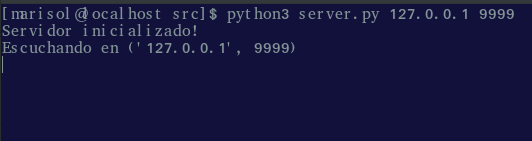
\includegraphics[width=0.7\linewidth]{1}
	\caption{Imagen de como se observa en la terminal el iniciar el servidor}
	\label{fig:1}
\end{figure}


\begin{itemize}
	\item Caso de Pokedex 
	
	Si queremos desplegar la pokedex de un usuario ejecutamos lo siguiente:
	
	\textsf{python3 server.py $<$IP$>$ $<$Puerto$>$ $<$Id\_usuario$>$ pokedex}
	
	%Imagen de pokedex
	\begin{figure}[h!]
		\centering
		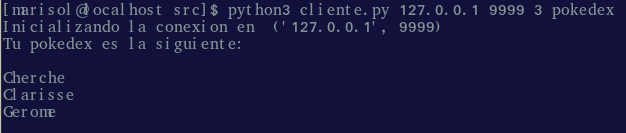
\includegraphics[width=0.7\linewidth]{pokedex}
		\caption{Captura de como se ve la pokedex}
		\label{fig:pokedex}
	\end{figure}
	
	
	\item Caso de atrapar pokemones
	
	Para este caso lo necesario es ejecutar lo siguiente: 
	
	\textsf{python3 server.py $<$IP$>$ $<$Puerto$>$ $<$Id\_usuario$>$}
	
	Si queremos atrapar a un pokemon el servidor nos dara un nombre de dicho pokemon y si queremos atraparlo. Al darle si correremos nuestro primer intento, en caso de no atraparlo nos dira los intentos restantes, y en caso de atraparlo nos mandara un mensaje indicando esto y desplegara la imagen de dicho pokemon.
	
	%imagen pokemon
	\begin{figure}
		\centering
		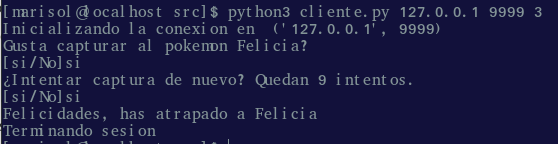
\includegraphics[width=0.7\linewidth]{Cachado1}
		\caption{Captura de la interaccion con el servidor al intentar obtener un pokemon.}
		\label{fig:cachado1}
	\end{figure}
	
	\begin{figure}[h!]
		\centering
		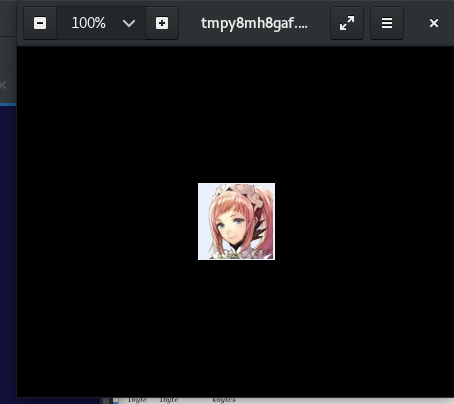
\includegraphics[width=0.4\linewidth]{cachado2}
		\caption{Captura de como se observa la imagen al capturar al pokemon.}
		\label{fig:cachado2}
	\end{figure}
	
\end{itemize}

En todos los casos el servidor nos dira que cliente entro y desde que puerto ademas de avisarnos cuando haya terminado de atender a un cliente.

\begin{figure}[h!]
	\centering
	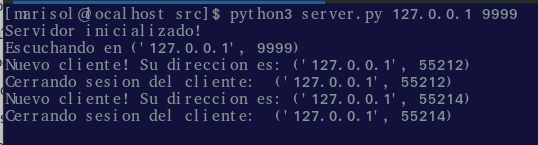
\includegraphics[width=0.7\linewidth]{servidorF}
	\caption{Captura de lo obtenido del servidor con la interaccion.}
	\label{fig:servidorf}
\end{figure}


\section{Requerimientos para la instalacion del proyecto}

Dado que esta desarrollado en Python es necesario tener Python 3 instalado y pip, para la base de datos de utilizo SQLite, por lo que sera necesario para las consultas de la base. Una vez con eso para instalar los modulos basta con ejecutar: 

	\textsf{pip install -r paquetes.txt}
	
	Esto instalara los paquetes necesarios, al final solo es necesario ejecutar los modulos como se explico anteriormente.
\end{document}